\section{Numerische Lösung nichtlinearer Gleichungssysteme}

\begin{remark}
    In diesem Kapitel geht es um die Nullstellenbestimmung von\\ nichtlinearen Funktionen $f: \R^n \to \R^n$. \\
    Abkürzung: LGS = lineares Gleichungssystem, NGS = nichtlineares Gleichungssystem
\end{remark}

\begin{example2}{Einleitendes Beispiel}
    $$f_1(x_1, x_2) = x_1^2 + x_2 - 11 = 0$$
    $$f_2(x_1, x_2) = x_1 + x_2^2 - 7 = 0$$
    Gesucht sind die Lösungen des Gleichungssystems. Diese lassen sich interpretieren als die Nullstellen der Funktion $\textbf{f}: \R^2 \to \R^2$ gemäss:
    $$\textbf{f}(x) = \begin{pmatrix} f_1 (x_1, x_2) \\ f_2 (x_1, x_2) \end{pmatrix} = \begin{pmatrix} x_1^2 + x_2 - 11 \\ x_1 + x_2^2 - 7 \end{pmatrix} = \begin{pmatrix} 0\\ 0 \end{pmatrix}$$
    Offensichtlich lässt sich ein solches System nicht in die Form $Ax = b$ bringen. 

    \begin{minipage}{0.5\linewidth}
    Geometrisch lassen sich die Lösungen als Schnittpunkte der beiden Funktionen interpretieren.\\
    Explizite Darstellung der Kurven:
    $$x_2 = 11 - x_1^2$$
    $$x_2 = \sqrt{7 - x_1}$$
    Schnittpunkte:
    $$\overline{\textbf{x}_1} = \begin{psmallmatrix} 3 \\ 2 \end{psmallmatrix}, \quad \overline{\textbf{x}_2} = \begin{psmallmatrix} -2.8 \\ 3.2 \end{psmallmatrix}$$
    $$\overline{\textbf{x}_3} = \begin{psmallmatrix} -3.8 \\ -3.3 \end{psmallmatrix}, \quad \overline{\textbf{x}_4} = \begin{psmallmatrix} 3.4 \\ -1.7 \end{psmallmatrix}$$
    \end{minipage}
    \begin{minipage}{0.5\linewidth}
    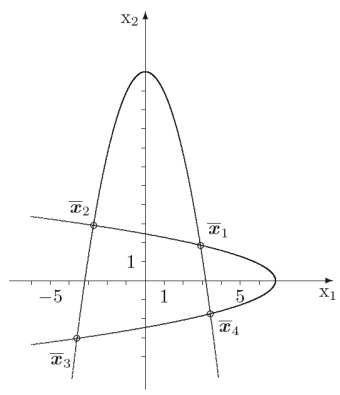
\includegraphics[width=\linewidth]{einleitendes_bsp_kap5.png}
    \end{minipage}
\end{example2}

\subsection{Funktionen mit mehreren Variablen}

\begin{lemma}{Funktion} mit abhängiger Variable $x$, unabhängiger Variable $y$ = $f(x)$:
    $$f: \R \to \R$$
    $$\quad x \mapsto f(x)$$
\end{lemma}

\begin{definition}{Skalarwertige Funktionen mit mehreren Variablen}
    $$f: D \subset \R^n \to W \subset \R$$
    $$(x_1, x_2, \ldots, x_n) \mapsto y = f(x_1, x_2, \ldots, x_n)$$
    Unter einer Funktion $f$ mit $n$ unabhängigen Variablen $x_1, \ldots, x_n$ und einer abhängigen Variablen $y$ versteht man eine Vorschrift, 
    die jedem geordneten Zahlentupel $(x_1, x_2, \ldots, x_n)$ aus einer Definitionsmenge $D \subset \R^n$ genau ein Element $y \in W \subset \R$ zuordnet.
    \vspace{2mm} \\
    Da das Ergebnis $y \in \R$ ein Skalar (eine Zahl) ist, redet man auch von einer \textbf{skalarwertigen Funktion}.
\end{definition}

\begin{concept}{Vektorwertige Funktion} Erweiterung der obigen Definition, gibt einen \textbf{Vektor} zurück (anstatt eines Skalars).\\
    Sei $\textbf{f}: \R^n \to \R^m$ eine Funktion mit $n$ Variablen. Dann ist die Funktion $\textbf{f}$ definiert durch:
    $$\textbf{f}(x_1 \ldots, x_n) = \begin{pmatrix} y_1 = f_1(x_1, x_2, \ldots, x_n) \\ y_2 = f_2(x_1, x_2, \ldots, x_n) \\ \vdots \\ y_m = f_m(x_1, x_2, \ldots, x_n) \end{pmatrix}$$
    wobei die $m$ Komponenten $f_i: \R^n \to \R$ für $i = 1, 2, \ldots, n$ von $\textbf{f}$ wieder \textbf{skalarwertige} Funktionen sind.
\end{concept}

\begin{corollary}{Eigenschaften von skalar- und vektorwertigen Funktionen}
    \begin{itemize}
        \item Skalar- und vektorwertige Funktionen mit mehreren Variablen werden auch \textbf{multivariat} genannt.
        \item Wie bei einem Vektor $\textbf{x}$ stellen wir zur besseren Unterscheidbarkeit vektorwertige Funktionen $\textbf{f}$ fett dar, im Gegensatz zu Skalaren $x$ und skalarwertigen Funktionen $f$.
        \item Wir werden uns bei der Lösung nichtlinearer Gleichungssysteme auf vektorwertige Funktionen $\textbf{f} = \R^n \to \R^n$ konzentrieren.
    \end{itemize}
\end{corollary}

\paragraph{Beispiele}

\begin{example2}{Grundlegende Rechenoperationen} können als Skalarwertige Funktionen $f: \R^2 \to \R$ oder als Vektorwertige Funktionen $\textbf{f}: \R^2 \to \R^2$ interpretiert werden
    $$f(x, y) = x + y, \quad g(x, y) = x \cdot y, \quad h(x, y) = x^2 + y^2$$
    $$\textbf{f}(x, y) = \begin{pmatrix} x + y \\ x \cdot y \end{pmatrix}, \quad \textbf{g}(x, y) = \begin{pmatrix} x \cdot y \\ x^2 + y^2 \end{pmatrix}$$
\end{example2}

\begin{example2}{Zusammenhang mit der Elektrotechnik}
    \paragraph{Ohmsches Gesetz}
    Die an einem ohmschen Widerstand $R$ abfallende Spannung $U$ hängt vom Widerstand $R$ und der Stromstärke $I$ gemäss dem ohmschen Gesetz $U=R \cdot I$ ab. Also haben wir für die abhängige Variable $U=f(R, I)=R I$ die skalarwertige Funktion $f: \mathbb{R}^2 \longrightarrow \mathbb{R}$ mit den unabhängigen Variablen $R$ und $I$. Häufig schreibt man auch direkt
    $$
    U=U(R, I)=R \cdot I
    $$
    und bringt dadurch die Abhängigkeit der Variable $U$ von den unabhängigen Variablen $R$ und $I$ zum Ausdruck, wie wir es auch bereits vom eindimensionalen Fall kennen, z.B. $y=y(x)$.

    \paragraph{Reihenschaltung von Widerständen}
    Bei der Reihenschaltung von $n$ ohmschen Widerständen $R_1, R_2, \ldots, R_n$ ergibt sich der Gesamtwiderstand $R$ gemäss
    $$
    R=R(R_1, R_2, \ldots, R_n)=R_1+R_2+\ldots+R_n
    $$    
\end{example2}

\begin{example2}{lineare Funktionen von LGS}
    Gebe die lineare Funktion $\textbf{f}: \R^3 \to \R^3$ an, für welche die Lösung $\textbf{x}$ des LGS:
    $$\textbf{Ax} = \textbf{b} \text{ mit } \textbf{A} = \begin{pmatrix} 4 & -1 & 1 \\ -2 & 5 & 1 \\ 1 & -2 & 5 \end{pmatrix} \text{ und } \textbf{b} = \begin{pmatrix} 1 \\ 2 \\ 3 \end{pmatrix}$$
    gerade $\textbf{f(x)} = \textbf{0}$ ergibt.
    \vspace{2mm} \\
    \textbf{Vorgehen}: \\
    $$\overrightarrow{\textbf{f}}(x_1, x_2, x_3) = 0 \begin{pmatrix} x_1 \\ x_2 \\ x_3 \end{pmatrix} = \begin{pmatrix} 0 \\ 0 \\ 0 \end{pmatrix}$$
    $$\textbf{A} \overrightarrow{\textbf{x}} = \overrightarrow{\textbf{b}} \Rightarrow \underbrace{\textbf{A} \overrightarrow{\textbf{x}} - \overrightarrow{\textbf{b}} = \overrightarrow{\textbf{0}}}_{\overrightarrow{\textbf{f}}(\overrightarrow{\textbf{x}})}$$
    \tcblower
    $$\overrightarrow{\textbf{f}}(\overrightarrow{\textbf{x}}) = \textbf{A} \overrightarrow{\textbf{x}} - \overrightarrow{\textbf{b}} = \begin{pmatrix} 4 & -1 & 1 \\ -2 & 5 & 1 \\ 1 & -2 & 5 \end{pmatrix} \begin{pmatrix} x_1 \\ x_2 \\ x_3 \end{pmatrix} - \begin{pmatrix} 5 \\ 11 \\ 12 \end{pmatrix}$$
    Die Funktion $\textbf{f}$ ist gegeben durch: (\textcolor{pink}{\textbf{solved by copilot so no guarantees}})
    $$\textbf{f}(x_1, x_2, x_3) = \begin{pmatrix} f_1 = 4x_1 - x_2 + x_3 - 5 \\ f_2 = -2x_1 + 5x_2 + x_3 - 11 \\ f_3 = x_1 - 2x_2 + 5x_3 - 12 \end{pmatrix}$$
\end{example2}

\subsubsection{Darstellungsformen}

\begin{concept}{Analytische Darstellung}
    \begin{itemize}
        \item \textbf{Explizite Darstellung:} $y = f(x_1, \ldots, x_n)$
        \begin{itemize}
            \item die Funktionsgleichung ist nach einer Variablen aufgelöst
            \item Beispiel: $y = 2 \cdot e^(x_1^2 + x_2^2)$
        \end{itemize}
        \item \textbf{Implizite Darstellung:} $F(x, y) = 0$
        \begin{itemize}
            \item die Funktionsgleichung ist nicht nach einer Variablen aufgelöst
            \item daher handelt es sich um eine Funktion mit nur $n-1$ unabhängigen Variablen
            \item Beispiel: $x_1^2 + x_2^2 - 1 = 0$
        \end{itemize}
        \item \textbf{Parameterdarstellung:} $x = x(t), y = y(t)$
        \begin{itemize}
            \item die Funktion wird durch eine Kurve im Raum beschrieben
            \item Beispiel: $x(t) = \cos(t), y(t) = \sin(t)$
        \end{itemize}
    \end{itemize}
\end{concept}

\begin{concept}{Darstellung durch Wertetabelle}
    Sei $f: \R^n \to \R^m$ eine Funktion.\\
    \textbf{Vorgehen:}\\
    In die vorausgesetzte Funktionsgleichung $z = f(x,y)$ werden die Werte der unabhängigen Variablen $x$ und $y$ eingesetzt (der Reihe nach).\\
    So erhält man eine Wertetabelle, bzw. Matrix:\\
    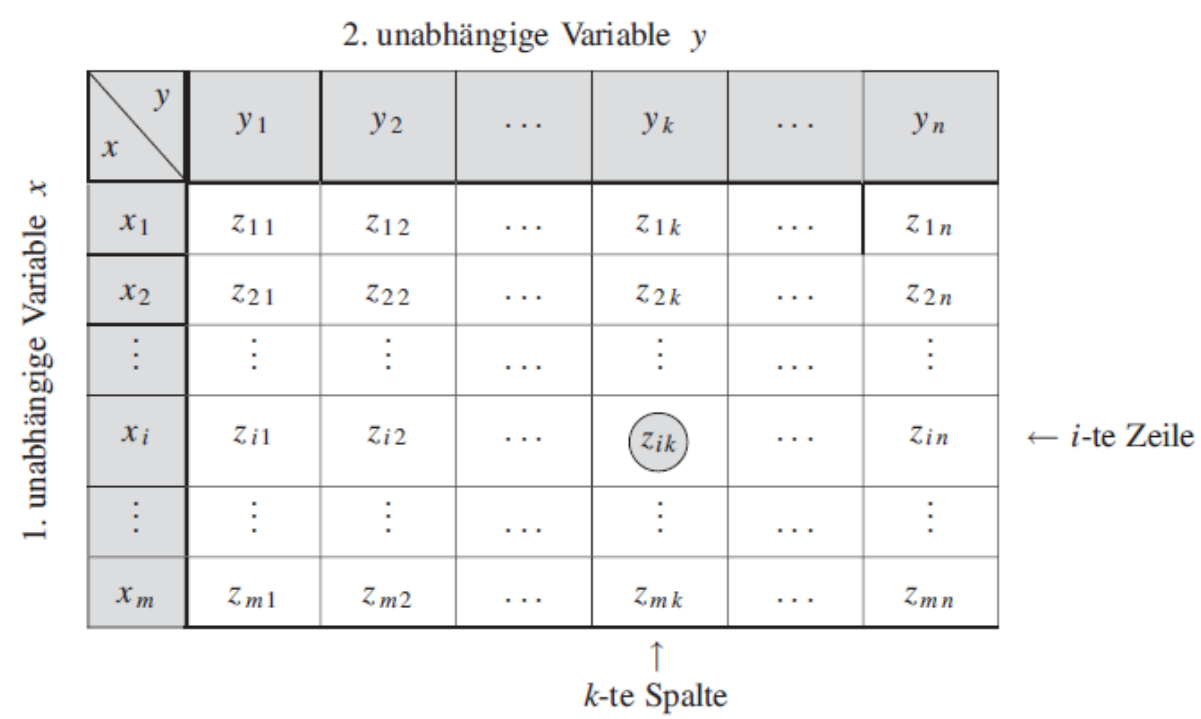
\includegraphics[width=\linewidth]{wertetabelle_darstellung.png}
\end{concept}

\begin{concept}{Grafische Darstellung}
    Wir beschränken uns hier auf skalarwertige Funktionen mit zwei unabhängigen Variablen $f: \R^2 \to \R$.\\
    Dazu betrachten wir die Funktion $z = f(x, y)$ in einem dreidimensionalen kartesischen Koordinatensystem:
    
    \paragraph{Darstellung einer Funktion als Fläche im Raum}
    Die Funktion $f$ ordnet jedem Punkt $(x, y) \in D$ in der Ebene einen Wert $z=f(x, y)$ zu, der als Höhenkoordinate verstanden werden kann. 
    Durch die Anordnung der Punkte ( $x, y, f(x, y)$ ) im dreidimensionalen Koordinatensystem wird eine über dem Definitionsbereich $D$ liegende Fläche ausgezeichnet:

    \includegraphics[width=\linewidth]{funktion_als_fläche_im_raum.png}
    
    \paragraph{Schnittkurvendiagramm}
    Wird die Fläche $z=f(x, y)$ bei einer konstanten Höhe $z=$ const. geschnitten, ergibt sich eine Schnittkurve. 
    Wird diese in die $(x, y)$-Ebene projiziert, spricht man von einer Höhenlinie bzw. bei der Abbildung von einem Höhenliniendiagramm., wie wir es z.B. von Wanderkarten her kennen. 
    Natürlich kann man auch andere Schnitte als $z=$ const. (Schnittebene parallel zur $(x, y)$-Ebene) wählen, z.B. $x=$ const. (Schnittebene parallel zur $(y, z)$-Ebene) oder $y=$ const. (Schnittebene parallel zur $(x, z)$-Ebene):

    \begin{minipage}{0.6\linewidth}
    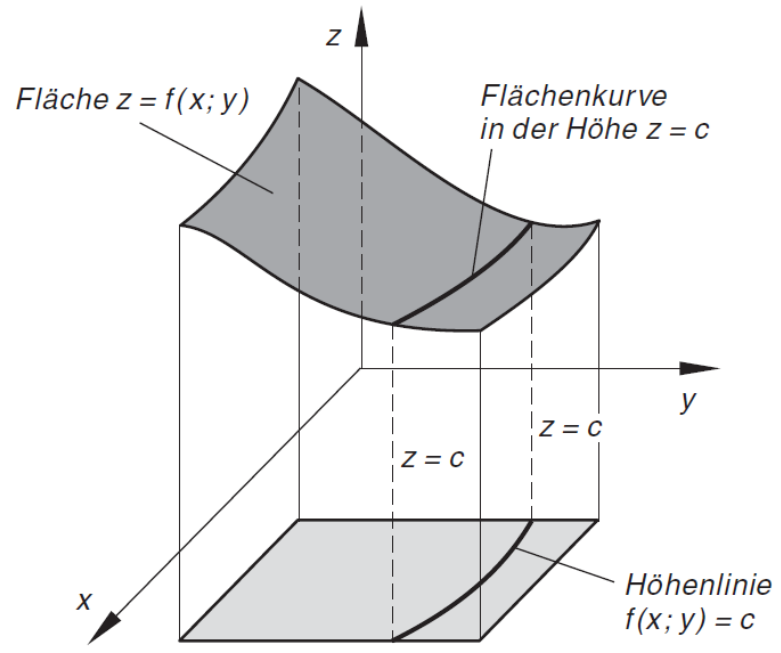
\includegraphics[width=\linewidth]{grafische_darstellung_detailed.png}
    \end{minipage}
    \begin{minipage}{0.38\linewidth}
    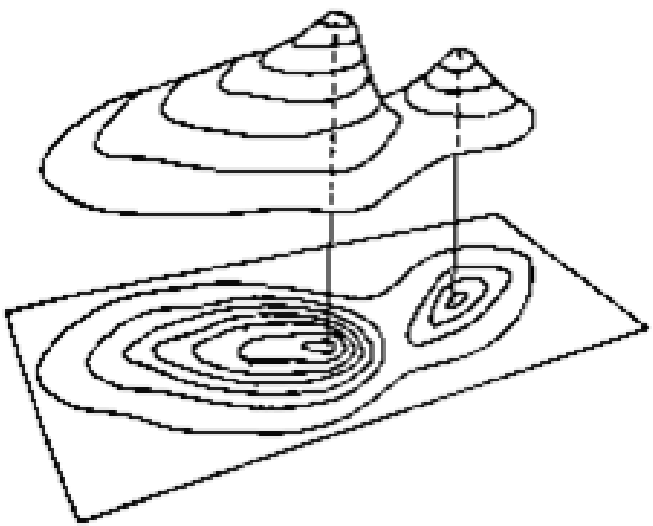
\includegraphics[width=\linewidth]{grafische_darstellung2.png}\\
    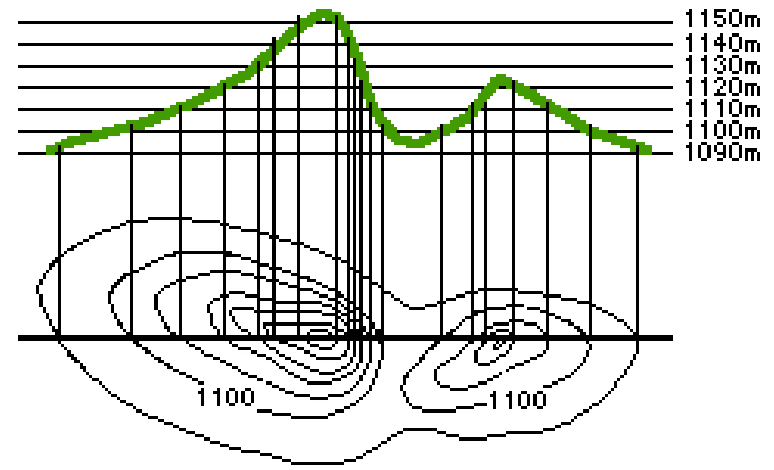
\includegraphics[width=\linewidth]{grafische_darstellung3.png}
    \end{minipage}
\end{concept}


\subsection{Partielle Ableitungen}

\begin{theorem}{Partielle Ableitung}
In einer Dimension
$$
f^{\prime}\left(x_0\right)=\lim _{\Delta x \rightarrow 0} \frac{\left(f\left(x_0+\Delta x\right)-f\left(x_0\right)\right)}{\Delta x}
$$

\textcolor{frog}{\textbf{In mehreren Dimensionen}}

1. Ableitung nach $x$ :
$$
f_x=\frac{\partial f}{\partial x}(x, y)=\lim _{\Delta x \rightarrow 0} \frac{f(x+\Delta x, y)-f(x, y)}{\Delta x}
$$
2. Ableitung nach $y: \quad f_y=\frac{\partial f}{\partial y}(x, y)=\lim _{\Delta y \rightarrow 0} \frac{f(x, y+\Delta y)-f(x, y)}{\Delta y}$
\end{theorem}

\begin{example}
$$
z=f(x, y)=3 x y^3+10 x^2 y+5 y+3 y \cdot \sin (5 x y)
$$

$$\frac{\partial f}{\partial x}(x, y)=3 \cdot 1 \cdot y^3+10 \cdot 2 x \cdot y+0+3 y \cdot \cos (5 x y) \cdot 5 \cdot 1 \cdot y$$
$$\frac{\partial f}{\partial y}(x, y)=3 x \cdot 3 y^2+10 x^2 \cdot 1+5 \cdot 1+(3 \cdot 1 \cdot \sin (5 x y)+3 y \cdot \cos (5 x y) \cdot 5 x \cdot 1)$$

Steigung der beiden Tangenten in $x-$ resp. $y$-Richtung im Punkt $\left(x_0, y_0\right)=(-1,1)$
\end{example}

\subsubsection{Linearisierung von Funktionen mit mehreren Variablen}

\begin{concept}{Jacobi-Matrix}\\
    Sei $f: \mathbb{R}^n \rightarrow \mathbb{R}^m$ mit $y=f(x)$ und $x=\left(x_1, x_2, \ldots, x_n\right)^T \in \mathbb{R}^n$. Die Jacobi-Matrix $D f(x)$ enthält sämtliche partiellen Ableitungen 1 . Ordnung von $f$.
    $$
    f(x)=\left(\begin{array}{c}
    y_1=f_1(x) \\
    y_2=f_2(x) \\
    \vdots \\
    y_m=f_m(x)
    \end{array}\right), \quad D f(x)=\left(\begin{array}{cllc}
    \frac{\partial f_1}{\partial x_1}(x) & \frac{\partial f_1}{\partial x_2}(x) & \cdots & \frac{\partial f_1}{\partial x_n}(x) \\
    \frac{\partial f_2}{\partial x_1}(x) & \frac{\partial f_2}{\partial x_2}(x) & \cdots & \frac{\partial f_2}{\partial x_n}(x) \\
    \vdots & \vdots & \ddots & \vdots \\
    \frac{\partial f_m}{\partial x_1}(x) & \frac{\partial f_m}{\partial x_2}(x) & \cdots & \frac{\partial f_m}{\partial x_n}(x)
    \end{array}\right)
    $$
\end{concept}

\begin{formula}{Verallgemeinerte Tangentengleichung}
    $$
    g(x)=f\left(x^{(0)}\right)+D f\left(x^{(0)}\right) \cdot\left(x-x^{(0)}\right)
    $$
    Beschreibt eine lineare Funktion und es gilt $f(x) \approx g(x)$ in einer Umgebung eines gegebenen Vektors $x^{(0)}=\left(x_1^{(0)}, x_2^{(0)}, \ldots, x_n^{(0)}\right)^T \in \mathbb{R}^n$. 
    Man spricht deshalb auch von der Linearisierung der Funktion $y=f(x)$ in einer Umgebung von $x^{(0)}$
    (ein hochgestellter Index in Klammern $x^{(k)}$ bezeichnet wie bisher einen Vektor aus $\R^n$ nach der $k$-ten Iteration).  
\end{formula}

\begin{definition}{Tangentialebene}\\
    Für den speziellen Fall $f: \mathbb{R}^2 \longrightarrow \mathbb{R}$ mit $y=f\left(x_1, x_2\right)$ und $\boldsymbol{x}^{(0)}=\left(x_1^{(0)}, x_2^{(0)}\right)^T \in \mathbb{R}^2$ 
    ist die Jacobi-Matrix nur ein Zeilenvektor mit zwei Elementen, nämlich:
    $$
    D f\left(x^{(0)}\right)=\left(\begin{array}{cc}
    \frac{\partial f}{\partial x_1}\left(x_1^{(0)}, x_2^{(0)}\right) & \frac{\partial f}{\partial x_2}\left(x_1^{(0)}, x_2^{(0)}\right)
    \end{array}\right)
    $$
    Dann liefert die Linearisierung
    $$
    \begin{aligned}
    g\left(x_1, x_2\right) & =f\left(x_1^{(0)}, x_2^{(0)}\right)+\left(\frac{\partial f}{\partial x_1}\left(x_1^{(0)}, x_2^{(0)}\right) \quad \frac{\partial f}{\partial x_2}\left(x_1^{(0)}, x_2^{(0)}\right)\right) \cdot\binom{x_1-x_1^{(0)}}{x_2-x_2^{(0)}} \\
    & =f\left(x_1^{(0)}, x_2^{(0)}\right)+\frac{\partial f}{\partial x_1}\left(x_1^{(0)}, x_2^{(0)}\right) \cdot\left(x_1-x_1^{(0)}\right)+\frac{\partial f}{\partial x_2}\left(x_1^{(0)}, x_2^{(0)}\right) \cdot\left(x_2-x_2^{(0)}\right)
    \end{aligned}
    $$
    die Gleichung der Tangentialebene.

    Sie enthält sämtliche im Flächenpunkt $\stackrel{\bullet}{P}=\left(x_1^{(0)}, x_2^{(0)}, f\left(x_1^{(0)}, x_2^{(0)}\right)\right)$ an die Bildfläche von $y=f\left(x_1, x_2\right)$ angelegten Tangenten.
\end{definition}

\begin{example}
    Beispiel: Linearisieren Sie für $x^{(0)}=(\pi / 4,0, \pi)^T$ der Funktion $f\left(x_1, x_2, x_3\right)$
    \vspace{2mm} \\
    1. Jacobi-Matrix $\operatorname{Df}\left(x_1, x_2, x_3\right)$ bilden
    $$
    f\left(x_1, x_2, x_3\right)=\binom{\sin \left(x_2+2 x_3\right)}{\cos \left(2 x_1+x_2\right)}, \quad D f\left(x_1, x_2, x_3\right)=\left(\begin{array}{ccc}
    0 & \cos \left(x_2+2 x_3\right) & \cos \left(x_2+2 x_3\right) \cdot 2 \\
    -\sin \left(2 x_1+x_2\right) \cdot 2 & -\sin \left(2 x_1+x_2\right) & 0
    \end{array}\right)
    $$

    2. Startvektor $x^{(0)}$ in Vektorwertige Funktion $f(x)$ und Jacobi-Matrix D $f(x)$ einsetzen
    $$
    f(\pi / 4,0, \pi)=f\left(x^{(0)}\right)=\binom{\sin (0+2 \pi)}{\cos (2 \cdot \pi / 4+0)}=\binom{0}{0}, \quad D f\left(x^{(0)}\right)=\left(\begin{array}{ccc}
    0 & 1 & 2 \\
    -2 & -1 & 0
    \end{array}\right)
    $$

    3. Verallgemeinerte Tangentengleichung
    $$
    g(x)=\underbrace{\binom{0}{0}}_{f\left(x_0\right)}+\underbrace{\left(\begin{array}{ccc}
    0 & 1 & 2 \\
    -2 & -1 & 0
    \end{array}\right)}_{D f\left(x_0\right)} \cdot \underbrace{\left(\begin{array}{c}
    x_1-\pi / 4 \\
    x_2-0 \\
    x_3-\pi
    \end{array}\right)}_{x-x_0}=\left(\begin{array}{ccc}
    x_2 & +2 x_3 & -2 \pi \\
    -2 x_1 & -x_2 & +\pi / 2
    \end{array}\right)
    $$
\end{example}

\subsection{Nullstellenbestimmung für NGS}

\begin{remark}
    Es gibt keine einfachen Methoden, um festzustellen, ob ein nichtlineares Gleichungssystem lösbar ist und wie viele Lösungen es hat. Deshalb entscheidet die Wahl
    einer «geeigneten Startnäherug» meist über erfolgt oder Misserfolg der eingesetzten numerischen Verfahren.
\end{remark}

\begin{concept}{Newton-Verfahren} \textcolor{pink}{?????}
    Das Newton-Verfahren ist ein iteratives Verfahren zur Bestimmung von Nullstellen einer Funktion. Es basiert auf der Linearisierung der Funktion um einen Startwert $x^{(0)}$.
    \begin{itemize}
        \item \textbf{Vorgehen:}
        \begin{enumerate}
            \item Startwert $x^{(0)}$ wählen
            \item Linearisierung der Funktion um $x^{(0)}$
            \item Nullstelle der Linearisierung berechnen
            \item Neue Linearisierung um die berechnete Nullstelle
            \item Iteration bis Konvergenz
        \end{enumerate}
        \item \textbf{Formel:}
        $$
        x^{(k+1)}=x^{(k)}-\left(D f\left(x^{(k)}\right)\right)^{-1} \cdot f\left(x^{(k)}\right)
        $$
    \end{itemize}
\end{concept}

\begin{concept}{Quadratisch konvergentes Newton-Verfahren} (Quadratische Konvergenz)
    
    Lösung von $f(x)=0$ mit $f: \mathbb{R}^n \rightarrow \mathbb{R}^n$ für $n=0,1,2, \ldots$
    \begin{enumerate}
        \item Berechne $f\left(x^{(n)}\right)$ und $D f\left(x^{(n)}\right)$
        \item Berechne $\delta^{(n)}$ als Lösung des lin. GS $D f\left(x^{(n)}\right) \cdot \delta^{(n)}=-f\left(x^{(n)}\right)$
        \item Setze $x^{(n+1)}:=x^{(n)}+\delta^{(n)}$
    \end{enumerate}
\end{concept}

\begin{theorem}{Vereinfachtes Newton-Verfahren} (Lineare Konvergenz)

    Lösung von $f(x)=0$ mit $f: \mathbb{R}^n \rightarrow \mathbb{R}^n$ für $n=0,1,2, \ldots$
    \begin{enumerate}
        \item Berechne $f\left(x^{(n)}\right)$ und $D f\left(x^{(0)}\right)$
        \item Berechne $\delta^{(n)}$ als Lösung des lin. GS $D f\left(x^{(0)}\right) \cdot \delta^{(n)}=-f\left(x^{(n)}\right)$
        \item Setze $x^{(n+1)}:=x^{(n)}+\delta^{(n)}$
    \end{enumerate}
\end{theorem}

\begin{corollary}{Gedämpftes Newton-Verfahren}

Nur in der Nähe der Nullstelle ist Konvergenz des Verfahrens garantiert!
\begin{enumerate}
    \item Berechne $f\left(x^{(n)}\right)$ und $D f\left(x^{(n)}\right)$
    \item Berechne $\delta^{(n)}$ als Lösung des lin. GS $D f\left(x^{(n)}\right) \cdot \delta^{(n)}=-f\left(x^{(n)}\right)$
    \item Finde das minimale $k \in\left\{0,1, \ldots, k_{\max }\right\}$ mit:
\end{enumerate}
$$
\left\|f\left(x^{(n)}+\frac{\delta^{(n)}}{2^k}\right)\right\|_2<\left\|f\left(x^{(n)}\right)\right\|_2
$$
Kein minimales $k$ gefunden $\rightarrow k=0$

4. Setze
$$
x^{(n+1)}:=x^{(n)}+\frac{\delta^{(n)}}{2^k}
$$
\end{corollary}


\begin{example2}{Beispiel mit Newton-Verfahren}
    
Gegeben sind zwei Gleichungen und der Start-Vektor $x^{(0)}=(2,-1)^T$

$$
1-x^2=y^2, \quad \frac{(x-2)^2}{a}+\frac{(y-1)^2}{b}=1
$$


Umwandlung in Funktionen $f_1, f_2=0$

$$
f_1(x, y)=1-x^2-y^2=0, \quad f_2(x, y)=\frac{(x-2)^2}{a}+\frac{(y-1)^2}{b}-1=0
$$


1: Vektorwertige Funktion und Jacobi-Matrix bilden

$$
D f(x, y)=\left(\begin{array}{cc}
-2 x & -2 y \\
\frac{2 x-4}{a} & \frac{2 y-2}{b}
\end{array}\right), \quad f(x, y)=\binom{1-x^2-y^2}{\frac{(x-2)^2}{a}+\frac{(y-1)^2}{b}-1}
$$


1: Start-Vektor $x^{(0)}$ einsetzen

$$
D f(2,-1)=\left(\begin{array}{cc}
-4 & 2 \\
0 & -4 / b
\end{array}\right), \quad f(2,-1)=\binom{-4}{4 / b-1}
$$


2: Berechne $\delta^{(0)}$

$$
\left(D f\left(x^{(0)}\right) \mid-f\left(x^{(0)}\right)\right)=\left(\begin{array}{cc|c}
-4 & 2 & 4 \\
0 & -4 / b & -4 / b+1
\end{array}\right) \rightarrow \underbrace{\binom{-1}{0}}_{\delta^{(0)}}
$$


3: Berechne $x^{(1)}$

$$
x^{(1)}=\underbrace{\binom{2}{-1}}_{x^{(0)}}+\underbrace{\binom{-1}{0}}_{\delta^{(0)}}=\binom{1}{-1}
$$
\end{example2}

\raggedcolumns

\section{Numerical Solution of Nonlinear Equation Systems}

\subsection{Introduction and Motivation}

\begin{definition}{Nonlinear Equation Systems}\\
A nonlinear equation system is a system of $n$ equations with $n$ unknowns that cannot be written in the form $Ax = b$ where $A$ is a matrix, $x$ is the vector of unknowns, and $b$ is a constant vector. Solving such systems requires finding values for variables that simultaneously satisfy all equations.
\end{definition}

\begin{example}
Consider the nonlinear system:
\begin{align*}
f_1(x_1, x_2) &= x_1^2 + x_2 - 11 = 0\\
f_2(x_1, x_2) &= x_1 + x_2^2 - 7 = 0
\end{align*}

This can be represented as finding the zeros of a vector-valued function $f: \mathbb{R}^2 \rightarrow \mathbb{R}^2$:
\begin{align*}
f(x) = \begin{pmatrix} x_1^2 + x_2 - 11 \\ x_1 + x_2^2 - 7 \end{pmatrix} = \begin{pmatrix} 0 \\ 0 \end{pmatrix}
\end{align*}

The geometric interpretation is finding the intersection points of two curves: $x_1^2 + x_2 = 11$ and $x_1 + x_2^2 = 7$.
\end{example}

\subsection{Functions of Several Variables}

\begin{definition}{Functions of Several Variables}\\
A function with $n$ independent variables $x_1, x_2, \ldots, x_n$ and one dependent variable $y$ is a mapping that assigns to each point $(x_1, x_2, \ldots, x_n)$ from a domain $D \subset \mathbb{R}^n$ exactly one element $y$ from a range $W \subset \mathbb{R}$.

We write: $f: D \subset \mathbb{R}^n \rightarrow W \subset \mathbb{R}$, $(x_1, x_2, \ldots, x_n) \mapsto y = f(x_1, x_2, \ldots, x_n)$
\end{definition}

\begin{definition}{Vector-Valued Functions}\\
A vector-valued function maps points from $\mathbb{R}^n$ to $\mathbb{R}^m$:
$f: \mathbb{R}^n \rightarrow \mathbb{R}^m$ with
$f(x_1, \ldots, x_n) = \begin{pmatrix} y_1 = f_1(x_1, x_2, \ldots, x_n) \\ y_2 = f_2(x_1, x_2, \ldots, x_n) \\ \vdots \\ y_m = f_m(x_1, x_2, \ldots, x_n) \end{pmatrix}$

Where the $m$ components $f_i: \mathbb{R}^n \rightarrow \mathbb{R}$ are scalar-valued functions.
\end{definition}

\subsubsection{Partial Derivatives}

\begin{definition}{Partial Derivatives}\\
For a function $z = f(x,y)$, the partial derivatives at the point $(x,y)$ are defined as:

\begin{align*}
\frac{\partial f}{\partial x}(x,y) &= \lim_{\Delta x \rightarrow 0} \frac{f(x+\Delta x, y) - f(x,y)}{\Delta x}\\
\frac{\partial f}{\partial y}(x,y) &= \lim_{\Delta y \rightarrow 0} \frac{f(x, y+\Delta y) - f(x,y)}{\Delta y}
\end{align*}

Alternative notations include: $f_x(x,y)$, $f_y(x,y)$ or $\frac{\partial f}{\partial x}$, $\frac{\partial f}{\partial y}$.

Geometrically, $\frac{\partial f}{\partial x}(x_0, y_0)$ represents the slope of the tangent to the surface $z=f(x,y)$ at the point $(x_0, y_0, z_0)$ in the positive $x$-direction, and similarly for $\frac{\partial f}{\partial y}(x_0, y_0)$ in the $y$-direction.
\end{definition}

\begin{example}
For the function $z = f(x,y) = 3xy^2 + \ln(x^3y^2)$, the partial derivatives are:
\begin{align*}
f_x &= 3 \cdot 1 \cdot y^2 + \frac{1}{x^3y^2} \cdot 3x^2 \cdot y^2 = 3y^2 + \frac{3y^2}{x}\\
f_y &= 3x \cdot 2y + \frac{1}{x^3y^2} \cdot x^3 \cdot 2y = 6xy + \frac{2}{y}
\end{align*}
\end{example}

\subsubsection{Linearization of Functions of Several Variables}

\begin{definition}{Jacobian Matrix and Linearization}\\
For a function $f: \mathbb{R}^n \rightarrow \mathbb{R}^m$ with $y = f(x) = \begin{pmatrix} y_1 = f_1(x) \\ \vdots \\ y_m = f_m(x) \end{pmatrix}$ and $x = (x_1, x_2, \ldots, x_n)^T \in \mathbb{R}^n$, the Jacobian matrix contains all first-order partial derivatives and is defined as:

\begin{align*}
Df(x) := \begin{pmatrix} 
\frac{\partial f_1}{\partial x_1}(x) & \frac{\partial f_1}{\partial x_2}(x) & \cdots & \frac{\partial f_1}{\partial x_n}(x) \\
\frac{\partial f_2}{\partial x_1}(x) & \frac{\partial f_2}{\partial x_2}(x) & \cdots & \frac{\partial f_2}{\partial x_n}(x) \\
\vdots & \vdots & \ddots & \vdots \\
\frac{\partial f_m}{\partial x_1}(x) & \frac{\partial f_m}{\partial x_2}(x) & \cdots & \frac{\partial f_m}{\partial x_n}(x)
\end{pmatrix}
\end{align*}

The linearization of $f$ at a point $x^{(0)}$ is given by:
\begin{align*}
g(x) = f(x^{(0)}) + Df(x^{(0)}) \cdot (x - x^{(0)})
\end{align*}
This gives a linear approximation of $f(x)$ in the neighborhood of $x^{(0)}$.
\end{definition}

\begin{example}
Consider $f(x_1, x_2) = \begin{pmatrix} x_1^2 + x_2 - 11 \\ x_1 + x_2^2 - 7 \end{pmatrix}$, linearized at $x^{(0)} = (1,1)^T$.

The Jacobian matrix is:
\begin{align*}
Df(x_1, x_2) = \begin{pmatrix} 2x_1 & 1 \\ 1 & 2x_2 \end{pmatrix}
\end{align*}

At the point $x^{(0)} = (1,1)^T$:
\begin{align*}
Df(1,1) = \begin{pmatrix} 2 & 1 \\ 1 & 2 \end{pmatrix}
\end{align*}

The linearization is:
\begin{align*}
g(x) &= f(x^{(0)}) + Df(x^{(0)}) \cdot (x - x^{(0)})\\
&= \begin{pmatrix} -9 \\ -5 \end{pmatrix} + \begin{pmatrix} 2 & 1 \\ 1 & 2 \end{pmatrix} \cdot \begin{pmatrix} x_1 - 1 \\ x_2 - 1 \end{pmatrix}\\
&= \begin{pmatrix} -9 + 2(x_1 - 1) + (x_2 - 1) \\ -5 + (x_1 - 1) + 2(x_2 - 1) \end{pmatrix}\\
&= \begin{pmatrix} 2x_1 + x_2 - 12 \\ x_1 + 2x_2 - 8 \end{pmatrix}
\end{align*}
\end{example}

\subsection{Newton's Method for Systems}

\begin{KR}{Newton's Method for Nonlinear Systems}\\
We seek to find zeros of a function $f: \mathbb{R}^n \rightarrow \mathbb{R}^n$.

\paragraph{Algorithm}
\begin{enumerate}
    \item Start with an initial guess $x^{(0)}$ close to a zero of $f$.
    \item For $n = 0, 1, 2, \ldots$ until convergence:
    \begin{itemize}
        \item Compute the correction $\delta^{(n)}$ by solving the linear system:
        
        $Df(x^{(n)})\delta^{(n)} = -f(x^{(n)})$
        
        \item Update the approximation:
        
        $x^{(n+1)} = x^{(n)} + \delta^{(n)}$
    \end{itemize}
    \item Convergence is achieved when a suitable stopping criterion is met, such as:
    \begin{itemize}
        \item $n \geq n_{max}$ (maximum iterations reached)
        \item $\|x^{(n+1)} - x^{(n)}\| \leq \epsilon\|x^{(n+1)}\|$ 
        \item $\|x^{(n+1)} - x^{(n)}\| \leq \epsilon$
        \item $\|f(x^{(n+1)})\| \leq \epsilon$
    \end{itemize}
\end{enumerate}

\paragraph{Convergence} 
Newton's method converges quadratically if the starting point is sufficiently close to a zero, $Df(x)$ is regular, and $f$ is three times continuously differentiable.
\end{KR}

\begin{example2}{Newton's Method Application}\\
Let's solve the system:
\begin{align*}
f(x_1, x_2) = \begin{pmatrix} 2x_1 + 4x_2 \\ 4x_1 + 8x_2^3 \end{pmatrix} = \begin{pmatrix} 0 \\ 0 \end{pmatrix}
\end{align*}

The Jacobian matrix is:
\begin{align*}
Df(x_1, x_2) = \begin{pmatrix} 2 & 4 \\ 4 & 24x_2^2 \end{pmatrix}
\end{align*}

Starting with $x^{(0)} = \begin{pmatrix} 4 \\ 2 \end{pmatrix}$:

1. Compute:
   \begin{align*}
   Df(4, 2) &= \begin{pmatrix} 2 & 4 \\ 4 & 96 \end{pmatrix}\\
   f(4, 2) &= \begin{pmatrix} 16 \\ 80 \end{pmatrix}
   \end{align*}

2. Solve the linear system:
   \begin{align*}
   \begin{pmatrix} 2 & 4 \\ 4 & 96 \end{pmatrix}\delta^{(0)} = -\begin{pmatrix} 16 \\ 80 \end{pmatrix}
   \end{align*}
   Yielding $\delta^{(0)} = \begin{pmatrix} -\frac{76}{11} \\ \frac{6}{11} \end{pmatrix}$

3. Update:
   \begin{align*}
   x^{(1)} = \begin{pmatrix} 4 \\ 2 \end{pmatrix} + \begin{pmatrix} -\frac{76}{11} \\ \frac{6}{11} \end{pmatrix} = \begin{pmatrix} -\frac{32}{11} \\ \frac{16}{11} \end{pmatrix} \approx \begin{pmatrix} -2.909 \\ 1.455 \end{pmatrix}
   \end{align*}

The sequence converges to $(-2, 1)^T$, one of the solutions.
\end{example2}

\subsubsection{Simplified Newton's Method}

\begin{definition}{Simplified Newton's Method}\\
To reduce computational effort per iteration, we can use the same Jacobian matrix for all iterations:

\begin{align*}
Df(x^{(0)})\delta^{(n)} = -f(x^{(n)})
\end{align*}

This method converges only linearly but requires fewer computations per step.
\end{definition}

\subsubsection{Damped Newton's Method}

\begin{KR}{Damped Newton's Method}\\
When the Jacobian matrix is nearly singular, the standard Newton step may cause the iterations to diverge. The damped Newton's method adjusts the step size to ensure convergence.

\paragraph{Algorithm}
\begin{enumerate}
    \item Start with an initial guess $x^{(0)}$ close to a zero of $f$.
    \item For $n = 0, 1, 2, \ldots$ until convergence:
    \begin{itemize}
        \item Compute $\delta^{(n)}$ by solving:
        
        $Df(x^{(n)})\delta^{(n)} = -f(x^{(n)})$
        
        \item Find the smallest $k \in \{0,1,\ldots,k_{max}\}$ such that:
        
        $\|f(x^{(n)} + \frac{\delta^{(n)}}{2^k})\|_2 < \|f(x^{(n)})\|_2$
        
        \item If no such $k$ is found, use $k = 0$
        
        \item Update:
        
        $x^{(n+1)} = x^{(n)} + \frac{\delta^{(n)}}{2^k}$
    \end{itemize}
\end{enumerate}

\paragraph{Notes}
\begin{itemize}
    \item The damping parameter $k_{max}$ is problem-dependent
    \item A value of $k_{max} = 4$ is often a good starting point
    \item Damped Newton's method generally converges more reliably than the standard method
\end{itemize}
\end{KR}

